%!TEX root=finmath1.tex
% \begingroup
% \renewcommand{\clearpage}{}
% \phantomsection
% \addcontentsline{toc}{chapter}{\textbf{Часть 1. Дискретное время}}
% \begin{center}
% \Large\bf \rule[1.5mm]{1cm}{1pt}\quad \textsc{Приложения}\quad \rule[1.5mm]{1cm}{1pt}
% \end{center}

\part{Дискретное время}

\chapter{Основные понятия. Одношаговая модель}
\label{ch:onestep}
\chaptertoc

В первом разделе этой лекции описываются основные идеи и задачи курса.
Далее рассматривается самая простая модель финансового рынка, на примере которой проще всего понять ключевые концепции финансовой математики.
% \endgroup

\section{Задача оценки производных финансовых инструментов}

Главная задача, изучаемая в этом курсе, заключается в вычислении цен производных финансовых инструментов на основе цен базовых инструментов.
В этом разделе мы кратко обсудим, чем производные инструменты отличаются от базовых, а также опишем принцип отсутствия арбитража "--- основную идею, используемую для нахождения цен производных инструментов.


\subsection{Базовые и производные инструменты}

\emph{Базовыми инструментами} или \emph{базовыми активами} называются финансовые инструменты, цены которых определяются фундаментальными факторами (прибыльностью компании, спросом на сырье и \td), а \emph{производными инструментами} "--- контракты, выплаты которых зависят от цен на базовые активы. 


\subsubsection{Базовые инструменты}

Примерами базовых инструментов являются акции компаний, фондовые индексы, иностранные валюты, товары, облигации, инструменты денежного рынка и др.
Кратко разберем основные из них.

\emph{Акция} "--- это ценная бумага, представляющая собой долю в собственности компании.
Владелец акции имеет право на получение дивидендов, а также на участие в управлении компанией.
Инвестирование в акции предполагает получение дохода в виде дивидендов, а также дохода или убытка, связанного с изменением цены акции. 

\emph{Фондовый индекс} является взвешенной суммой цен активов, входящих в него.
Индекс служит как индикатором состояния рынка, так и может использоваться для расчета цен производных инструментов, таких как фьючерсы и опционы на индекс.
Известными индексами являются S\&P 500, NASDAQ и DJIA (США), EURO STOXX 50 (Европа), FTSE 100 (Великобритания), Nikkei 225 (Япония), IMOEX (Россия) и др.

\emph{Товары}, которые торгуются на рынках, включают металлы (золото, серебро), энергоносители (нефть, газ), сельскохозяйственную продукцию (пшеница, сахар) и др.
Ключевым свойством товаров, которые могут торговаться на организованных рынках, является возможность стандартизации их качества и количества (например, баррель нефти сорта Brent). 

\emph{Облигация} "--- это ценная бумага, представляющая собой долговое обязательство по возврату определенной денежной суммы.
Облигации выпускаются государством или компаниями для финансирования своей деятельности.
Владелец облигации имеет право на получение процентов по облигации (купонов) и возврат номинальной стоимости облигации по истечении срока.

\emph{Денежный рынок} состоит из краткосрочных финансовых инструментов сроком до 1 года.
Сюда можно отнести краткосрочные облигации, векселя, сделки репо и подобные инструменты.

Что касается математических моделей, то в нашем курсе будут два абстрактных класса инструментов: \emph{рисковые активы} и \emph{безрисковые активы}.
Первый является собирательной моделью для акций, индексов, валют, товаров; второй "--- для инструментов денежного рынка и, отчасти, облигаций. 


\subsubsection{Производные финансовые инструменты}

Производные инструменты "--- это контракты, выплаты по которым зависят от цен базовых инструментов, на основе которых они заключены. 
Существует множество различных производных финансовых инструментов, торгуемых как на организованных рынках (биржах), так и вне биржевых торгов.
В качестве основного примера рассмотрим \emph{опционы}.

\emph{Опцион колл} дает покупателю опциона право на покупку определенного количества базового актива по фиксированной цене (\emph{цена исполнения} или \emph{цена страйк}) в определенный момент времени (\emph{момент экспирации}).
Продавец опциона обязан выполнить требование покупателя в случае его предъявления и продать базовый актив.
За приобретение опциона покупатель платит продавцу вознаграждение (\emph{цену опциона} или \emph{премию}) в момент заключения контракта%
\footnote{Расчеты по опционам, обращающимся на биржах, происходят не непосредственно между покупателем и продавцом, а через клиринговый центр.
Для математической теории эта деталь несущественна.}.

\emph{Опцион пут} дает покупателю опциона право на продажу определенного количества базового актива по фиксированной цене в определенный момент времени.
Продавец опциона обязан выполнить требование покупателя в случае его предъявления и купить базовый актив. 

Опционы позволяют инвесторам защитить свои позиции от неблагоприятных изменений цен, а также могут использоваться для спекуляции на изменениях как самих цен базовых активов, так и производных от них характеристик (например, рыночной \emph{волатильности}).

Перечислим некоторые характеристики, по которым могут различаться опционы, помимо базового актива, страйка и времени исполнения. 
\begin{itemize}
\item По типу выплаты: \emph{ванильные}%
\footnote{Ванильный "--- синоним слова <<простой>>.}
(как выше) или \emph{экзотические} (например, опционы с барьером, опционы с автоколлом и др.).

\item По типу исполнения: \emph{европейские} (с возможностью предъявления к исполнению только в момент экспирации) или \emph{американские}%
\footnote{Это вовсе не означает, что европейские опционы торгуются только в Европе, а американские "--- только в Америке.}
(с возможностью предъявления к исполнению в любой момент времени до экспирации).

\item \emph{Расчетные} или \emph{поставочные}: в первом случае опционные выплаты происходят в денежной форме (продавец платит покупателю разницу в цене в момент исполнения, если эта разница положительна), во втором происходит передача базового актива.

% \item \emph{Премиальные} или \emph{маржируемые}.
% В премиальных опционах покупатель выплачивает продавцу премию (цену опциона) в момент покупки опциона и получает право исполнить опцион.
% В маржируемых опционах используется более сложный механизм ежедневного перечисления \emph{вариационной маржи}, равной изменению стоимости опциона за день.
\end{itemize}

В этом курсе, в основном, мы будем рассматривать только ванильные европейские опционы.
Во всех моделях без ограничения общности можно будет предполагать, что опционы являются расчетными (точнее говоря, цены расчетных и поставочных опционов будут совпадать).
Американские опционы обсуждаются в лекции \ref{ch:american-discrete}.

Центральной темой курса будет задача определения \emph{справедливых цен} опционов и других производных инструментов. 

\begin{example}
На бирже CBOE (Chicago Board Options Exchange "--- крупнейшая опционная биржа) опцион пут на индекс S\&P 500 со страйком 5840 и датой исполнения 21.03.2025 имел цену \$132.2--\$133.0 (цены лучших заявок на покупку и продажу на момент закрытия торгов)%
\footnote{\url{https://www.cboe.com/delayed_quotes/spx/quote_table}.} на дату 13.01.2025.
Значение индекса S\&P 500 к моменту закрытия торгов в тот день было 5836.
Опцион является европейским и расчетным. 

Если на момент экспирации значение индекса будет ниже 5840, то покупатель опциона получит прибыль, равную разнице между ценой страйк и значением индекса. Если значение индекса превысит 5840, то покупатель опциона не получит ничего. Издержки покупателя в обоих случаях будут равны цене, по которой он купил опцион.
\end{example}




\subsection{Принцип безарбитражности}
\subsubsection{Что такое арбитраж}

\index{арбитраж}
\emph{Арбитраж} -- это возможность получить прибыль без начальных вложений капитала и не неся риск. 
\emph{Принцип отсутствия арбитража} (также говорят \emph{гипотеза} отсутствия арбитража) "--- это предположение о том, что на рынке не существует арбитражных возможностей. 

Например, арбитражем является следующая схема: взять в долг \${$x$}, купить на эту сумму какой-то актив, а затем продать его в будущем по цене, заведомо превышающей \${$x$} плюс проценты по долгу.
Начальные вложения здесь нулевые, \tk\ актив покупается на заемные деньги, а прибыль положительна, \tk\ рост цены компенсирует проценты по долгу. 
Если бы такая возможность существовала, то многие участники рынка захотели бы ей воспользоваться.
Это бы неизбежно привело к росту спроса на актив и росту его цены, в результате чего арбитражная возможность бы пропала. 

В теории считается, что на эффективно работающих рынках арбитраж невозможен%
\footnote{Говоря более точно, считается, что арбитражные возможности исчезают настолько быстро, что ими нельзя воспользоваться  в рамках той теории, которая излагается в этом курсе.},
и, следовательно, принцип отсутствия арбитража является разумным предположением.
На основе этого предположения построена вся теория оценки производных инструментов.


\subsubsection{Безарбитражные цены}

Минимальное требование, которое предъявляется к цене производного инструмента, состоит в том, что цена не должна вносить арбитраж на рынок.
Такая цена называется \emph{безарбитражной}.
Поясним на примере простой модели.

\begin{example}
Пусть в момент времени $t=0$ акция стоит \$100, а в момент времени $t=1$ может стоить \$110 или \$90 (всего две возможности).
Предположим также, что процентная ставка на денежном рынке равна нулю, \te\ можно свободно брать деньги в долг, а депозит не приносит дохода.
Рассмотрим опцион пут со страйком \$100, который можно исполнить в момент $t=1$.
Если цена акции будет \$90, то покупатель опциона получит прибыль \$10.
Если цена будет \$110, то покупатель получит нулевую прибыль.
Какая будет безарбитражная стоимость опциона?

Сразу отметим, что неправильно считать ее равной математическому ожиданию прибыли. 
Во-первых, нам не даны вероятности цен в момент $t=1$.
Во-вторых, даже если бы они были известны (например, из статистики прошлых цен), то, как мы увидим далее, они не имеют отношения к вычислению безарбитражной цены.

Оказывается, безарбитражная цена равна \$5.
Ключевое соображение состоит в том, что выплату по данному опциону можно \emph{реплицировать} портфелем, состоящим из $-0.5$ акции и \$55.
Отрицательное количество акций означает \emph{короткую продажу} (взятие актива в долг); также в наших моделях будет считаться, что можно покупать и продавать дробное число акций.
Репликация означает, что стоимость этого портфеля в момент $t=1$ в точности равна выплате по опциону, \te\ \$0 или \$10 в зависимости от цены акции ($-0.5 \cdot 110 + 55 =0$ и $-0.5 \cdot 90 + 55 = 10$).

Такой портфель стоит \$5 в момент $t=0$ ($-0.5 \cdot 100 + 55 = 5$).
Если бы рыночная цена опциона была выше \$5, то можно было бы продать опцион и купить реплицирующий портфель.
Разность цен будет прибылью, а риска не будет, так как выплата по опциону компенсируется стоимостью продажи портфеля.
Если бы цена была ниже \$5, то можно продать портфель (взять его со знаком минус: взять в долг \$55 и купить 0.5 акции) и купить опцион.
Позиция в портфеле будет стоить \$0 или $-$\$10 в момент $t=1$, и ее можно покрыть выплатой по опциону.
Лишь при цене опциона \$5 арбитража не возникает. 
\end{example}


\section{Одношаговая биномиальная модель рынка}

Будем рассматривать модель, в которой рынок функционирует в два момента времени, $t=0$ (<<сегодня>>) и $t=1$ (<<завтра>>).
Вся случайность описывается множеством исходов $\Omega=\{\omega_u, \omega_d\}$, где <<u>>, <<d>> соответствуют тому, что цена акции пойдет вверх или вниз%
\footnote{Это не совсем строго, так как если, например, $d>0$, то цена идет вверх в обоих случаях, но для удобства будем говорить именно <<вверх>> и <<вниз>>.}. 

В модели имеются два актива: \emph{безрисковый} и \emph{рисковый}.
Безрисковый актив характеризуется процентной ставкой $r>-1$.
Сумма денег $x$, вложенная в него сегодня, превратится в $(1+r)x$ завтра.

Рисковый актив характеризуется ценой $S_0$ сегодня и ценой
$S_1(\omega)$ завтра.
Будем обозначать $s_u = S_1(\omega_u)$ и $s_d= S_1(\omega_d)$.
Без ограничения общности считаем, что $s_u>s_d$. 
Удобно также ввести в обозначения параметры $u,d$ такие, что $s_u = (1+u)S_0$ и $s_d = (1+d) S_0$. 
Возможные изменения цены акции схематично изображены на рис.~\ref{os:f:price}.

\begin{figure}[h]
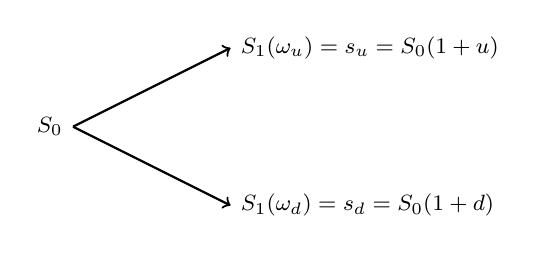
\begin{tikzpicture}
\draw[thick,->] (0,0) node[left] {\footnotesize $S_0$} 
  -- (2,1) node[right] {\footnotesize $S_1(\omega_u) = s_u = S_0(1+u)$};
\draw[thick,->] (0,0) 
  -- (2,-1) node[right] {\footnotesize $S_1(\omega_d) = s_d = S_0(1+d)$};
\end{tikzpicture}
\centering
\caption{Динамика цены акции в одношаговой модели.}
\label{os:f:price}  
\end{figure}

Таким образом, вся модель задается 4 параметрами $S_0,r,u,d$. Параметр $S_0$ положительный, а параметры $r$, $u$, $d$ больше $-1$.

\emph{Торговой стратегией} (или \emph{портфелем}) будем называть пару $\pi=(G,H)$, где $G$ выражает количество денежных единиц, вложенных в безрисковый актив, в момент времени $t=0$, а $H$ "--- количество акций, купленных в момент $t=0$.
Величины $G$ и $H$ могут быть как положительными, так и отрицательными (отрицательное количество денег означает взятие в долг, отрицательное количество акций -- короткую продажу); они также могут быть дробными. 

\emph{Стоимость портфеля $\pi$} сегодня по определению равна $V_0^\pi = G + HS_0$, а стоимость завтра равна $V_1^\pi(\omega) = G(1+r) + H S_1(\omega)$.
Изменение стоимости портфеля изображено на рис.~\ref{os:f:portfolio}.

\begin{figure}[h]
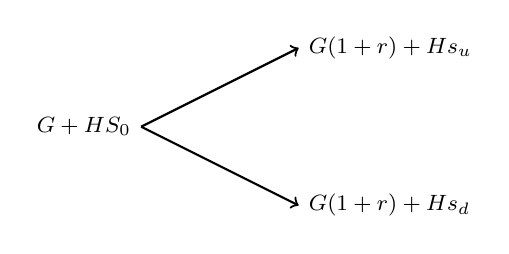
\begin{tikzpicture}
\draw[thick,->] (0,0) node[left] {\footnotesize $G+HS_0$} 
  -- (2,1) node[right] {\footnotesize $G(1+r) + Hs_u$};
\draw[thick,->] (0,0) --  (2,-1) node[right] {\footnotesize $G(1+r) + Hs_d$};
\end{tikzpicture}
\centering
\caption{Динамика стоимости портфеля в одношаговой модели.}
\label{os:f:portfolio}  
\end{figure}

\emph{Производный финансовый инструмент} (синоним -- \emph{платежное обязательство}) в такой модели представляется случайной величиной $X(\omega)$, которая задает сумму денег, которую \emph{продавец} этого инструмента выплачивает \emph{покупателю}%
\footnote{Названия сторон <<покупатель>> и <<продавец>> в такой абстрактной постановке весьма условны: если значение $X$ отрицательно, то, по сути, покупатель платит продавцу.}
в момент времени $t=1$. В свою очередь, покупатель покупает такой инструмент у продавца в момент времени $t=0$ за цену $V^X$.

Нашей задачей будет найти справедливую величину $V^X$.


\section{Цены платежных обязательств в одношаговой модели}

\subsection{Цена репликации}

\begin{definition}
Портфель $\pi$ \emph{реплицирует} платежное обязательство $X$, если $V_1^\pi(\omega) = X(\omega)$ для обоих исходов $\omega=\omega_u,\omega_d$. 
\end{definition}

\begin{proposition}
В одношаговой биномиальной модели для любого платежного обязательства существует единственный реплицирующий портфель.
\end{proposition}

\begin{proof}
Обозначим $x_u=X(\omega_u)$, $x_d=X(\omega_d)$.
Условие репликации эквивалентно системе линейных уравнений
\begin{equation}
\label{os:replication}
\left\{
\begin{aligned}
&G(1+r) + Hs_u = x_u,\\
&G(1+r) + Hs_d = x_d,
\end{aligned}\right.
\end{equation}
где $G$ и $H$ являются неизвестными.
В силу предположения $s_u>s_d$ решение этой системы существует и единственно.
\end{proof}

\begin{definition}
\emph{Ценой репликации} платежного обязательства $V^X$ называется стоимость $V^\pi_0$ соответствующего реплицирующего портфеля. 
\end{definition}

Найдем цену репликации в явном виде.
Решая систему \eqref{os:replication}, получаем, что реплицирующий портфель задается формулой
\label{os:replication-portfolio}
\[
G = \frac{1}{1+r} \cdot \frac{x_d s_u - x_us_d}{s_u - s_d}, \qquad
H = \frac{x_u-x_d}{s_u-s_d}.
\]
Теперь, учитывая, что $s_u = (1+u)S_0$, $s_d = (1+d)S_0$, находим
\[
V^X = G + HS_0 = \frac{1}{1+r}\cdot \frac{x_u(r-d) + x_d(u-r)}{u-d}.
\]

Как обсуждалось в первом разделе, цена репликации справедлива в том смысле, что она не приводит к возникновению арбитража (более точно, что такое арбитраж, мы определим далее). Поэтому естественно считать справедливой ценой платежного обязательства его цену репликации.


\subsection{Оценка с помощью риск-нейтральной вероятности}

Покажем, что цену репликации можно представить в виде математического ожидания относительно специально подобранной вероятности.

\begin{definition}
Вероятность $Q$ на множестве исходов $\Omega=\{\omega_u,\omega_d\}$ называется \emph{риск-нейтральной} если $Q(\omega_u) > 0$, $Q(\omega_d) > 0$ и $\E^Q {S_1}= (1+r)S_0$, где $\E^Q$ обозначает математическое ожидание по этой вероятности%
\footnote{То есть для случайной величины $\xi$ имеем $\E^Q \xi = \xi(\omega_u) Q(\omega_u) + \xi(\omega_d) Q(\omega_d)$.}.
\end{definition}

Название <<риск-нейтральная>> происходит из того, что цена акции сегодня будет равна ожиданию дисконтированной \emph{линейной полезности} от цены завтра по вероятности $\Q$: $S_0 = \E^Q u(S_1)/(1+r)$, где $u(x) = x$.
Экономические агенты, использующие линейную функцию полезности, считаются нейтральными к риску, что и объясняет название.

\begin{proposition}
\label{os:t:emm}
В одношаговой биномиальной модели риск-нейтральная вероятность существует тогда и только тогда, когда $d<r<u$.
Если она существует, то она единственна и задается формулой
\[
Q(\omega_u) = \frac{r-d}{u-d}, \qquad
Q(\omega_d) = \frac{u-r}{u-d}.
\]
\end{proposition}

\begin{proof}
Часть <<тогда>> и единственность $Q$ вытекают из того, что следующая система уравнений имеет единственное решение $(q_u,q_d)$ со строго положительными величинами $q_u$, $q_d$, которые соответствуют значениям $Q(\omega_u)$ и $Q(\omega_d)$:
\[
\left\{
\begin{aligned}
&(1+r)S_0 = s_dq_d + s_uq_u,\\
&q_u + q_d = 1.\\
\end{aligned}
\right.
\]
Первое уравнение здесь появляется из определения риск-нейтральной вероятности, а второе из того, что сумма вероятностей должна давать единицу.

Для доказательство части <<только тогда>> предположим, от противного, что $Q$ существует, но $r\le d < u$. Тогда
\[
\E^Q S_1 = s_d q_d + s_uq_u > (1+r)S_0 q_d + (1+r)S_0 q_u = (1+r)S_0.
\]
Наличие строго неравенства в этой формуле приводит к противоречию с определением $Q$.
Аналогично показывается, что и случай $d<u\le r$ невозможен.
\end{proof}

\begin{proposition}
Пусть $d < r< u$. Тогда для любого портфеля $\pi$ выполнено равенство
\[
V_0^\pi = \E^Q \frac{V_1^\pi}{1+r}.
\]
В частности, цену любого платежного обязательства $X$ можно найти как
\begin{equation}
\label{os:risk-neutal-price}
V^X = \E^Q \frac{X}{1+r}.
\end{equation}
\end{proposition}

\begin{proof}
Первое утверждение следует из цепочки равенств  
\[
\E^Q \frac{V_1^\pi}{1+r} = \E^Q \biggl(\frac{G(1+r) + HS_1}{1+r}\biggr) 
= G + H\E^Q\frac{S_1}{1+r} = G + HS_0 = V_0^\pi.
\]
Второе утверждение верно в силу того, что если портфель $\pi$ реплицирует $X$, то $X = V_1^\pi$ и $V^X = V_0^\pi$.
\end{proof}


\subsection{Отсутствие арбитража}

Рассмотрим подробнее условие $d<r<u$.
Оно означает, что доходность по безрисковому активу должна лежать строго между доходностью по акции в двух случаях $\omega_u$ и $\omega_d$.
Если это условие не выполнено, то инвестирование в один из активов оказывается заведомо менее прибыльным, чем в другой.
Покажем, что это приводит к арбитражу и, следовательно, в реалистичной модели всегда должно быть $d<r<u$.

\begin{definition}
\emph{Арбитражной возможностью} называется портфель $\pi$ со свойствами
\begin{alphenum}
\item $V_0^\pi = 0$,
\item $V_1^\pi(\omega) \ge 0$ для обоих исходов $\omega_u$, $\omega_d$,
\item $V_1^\pi(\omega) > 0$ хотя бы для одного из исходов $\omega_u$, $\omega_d$.
\end{alphenum}
\end{definition}
Первое условие означает, что для реализации арбитражной возможности не требуется начальных вложений капитала. Второе условие означает, что арбитражная возможность не несет риска. Третье условие "--- что она дает прибыль хотя бы в одном из исходов.

\begin{definition}
\emph{Гипотеза отсутствия арбитража NA} (no arbitrage) состоит в том, что в модели рынка нет арбитражных возможностей. 
\end{definition}

В финансовой математике считается, что во всех рассматриваемых моделях не должно быть арбитража, \te\ должна быть выполнена гипотеза NA.

\begin{proposition}
\label{os:ftap}
В одношаговой биномиальной модели выполнение гипотезы NA эквивалентно условию $d<r<u$, и, следовательно, эквивалентно существованию риск-нейтральной вероятности.
\end{proposition}

\begin{proof}
Пусть выполнено неравенство $d<r<u$. Тогда, согласно предложению \ref{os:t:emm}, существует риск-нейтральная вероятность $Q$.
Предположим, от противного, что существует арбитражная возможность $\pi$. Тогда 
\[
0 = V_0^\pi = \E^Q\frac{V_1^\pi}{1+r} 
= \frac{1}{1+r}( V_1^\pi(\omega_u) Q(\omega_u) + V_1^\pi(\omega_d) Q(\omega_d)) > 0.
\]
В последнем неравенстве воспользовались тем, что $V_1^\pi\ge 0$, причем хотя бы одно из значений $V_1^\pi(\omega_u)$ или $V_1^\pi(\omega_d)$ строго положительно, а кроме того обе вероятности $Q(\omega_u)$ и $Q(\omega_d)$ строго положительны.
Получаем противоречие: $0>0$.
Следовательно, арбитражная возможность не может существовать.

В обратную сторону: если $r\le d < u$, то нетрудно проверить, что $\pi = (-S_0,1)$ является арбитражной возможностью. Если же $d <u  \le r$, то $\pi = (S_0,-1)$ будет арбитражной возможностью.
В итоге, если арбитража нет, то должно быть выполнено неравенство $d<r<u$. 
\end{proof}

\begin{remark}
Предложение~\ref{os:ftap} является частным случаем \emph{первой фундаментальной теоремы финансовой математики}.
В общем виде она утверждает, что безарбитражность рынка равносильна существованию \emph{эквивалентной мартингальной меры}.
Для одношаговой биномиальной модели найденная нами риск"=нейтральная вероятность и есть такая мера. Общий случай мы обсудим позднее в курсе.
\end{remark}


\section{Примеры оценки платежных обязательств}

\subsection{Бескупонная облигация}
В одношаговой биномиальной модели \emph{бескупонная облигация}%
\footnote{В одношаговой модели нет смысла говорить о купонах, так как нет промежуточных моментов времени.}
соответствует платежному обязательству с константной выплатой $X$. 
Величина $X$ называется \emph{номиналом} (номинальной стоимостью) облигации.
Покажем, что цена такой облигации равна
\[
V^X = \frac{X}{1+r}.
\]

\textit{Первый способ (репликация).}
Выплату $X$ можно реплицировать портфелем $\pi=(G,H)$, где $G = X/(1+r)$ и $H=0$. Ясно, что $V^\pi_0 = G = X/(1+r)$.

\textit{Второй способ (риск-нейтральная оценка).}
По формуле \eqref{os:risk-neutal-price} имеем
\[
V^X = \E^Q \frac{X}{1+r} = \frac{X}{1+r},
\]
где воспользовались тем, что выражение под знаком ожидания есть константа.

\subsection{Форвардный контракт и форвардная цена}
По определению, \emph{форвардным контрактом} (или просто \emph{форвардом}) называется контракт на покупку базового актива по заранее установленной цене: покупатель форварда обязуется купить актив по цене $F$ в определенный момент времени, а продавец обязуется продать этот актив.

В одношаговой модели форвард соответствует платежному обязательству $X = S_1 - F$.
Так как в момент времени $t=0$ расчеты между сторонами не происходят, то  справедливое значение величины $F$ должно быть выбрано из условия $V^X=0$. Такое $F$ называется \emph{форвардной ценой} базового актива.
Покажем, что 
\[
F = (1+r) S_0.
\]

\textit{Первый способ (репликация).} Портфель $\pi=(G,H)$, где $G = -F/(1+r)$, $H=1$, реплицирует обязательство $X=S_1 - F$ для любого значения $F$. Начальная стоимость $V_0^\pi = S_0 - F/(1+r)$.
Тогда из условия $V^\pi_0 = 0$ находим $F=(1+r)S_0$.

\textit{Второй способ (риск-нейтральная оценка).} По формуле \eqref{os:risk-neutal-price} имеем
\[
V^X = \E^Q \frac{S_1 - F}{1+r} = \E^Q\frac{S_1}{1+r} - \frac{F}{1+r} = S_0 - \frac{F}{1+r},
\]
где во втором равенстве воспользовались определением риск-нейтральной вероятности ($\E^Q S_1/(1+r) = S_0$) и тем, что $F$ "--- константа.
Приравнивая $V^X_0$ к нулю, получаем такое же выражение для $F$, как и в способе с репликацией.

\subsection{Опционы колл и пут}
Европейские опционы колл и пут можно отождествить с платежными обязательствами
\[
X^c = (S_1 - K)^+, \qquad X^p = (K - S_1)^+,
\]
где запись $x^+$ означает $\max(x,0)$.
Действительно, если $S_1(\omega) > K$, то покупатель опциона колл получит выплату $S_1(\omega) - K$, а если $S_1(\omega) < K$, то выплаты не будет; кратко это можно записать как $(S_1 - K)^+$.
Аналогично для опциона пут.

Цены опционов вычисляются по формулам
\[
C =  \E^Q \frac{(S_1 - K)^+}{1+r}, \qquad
P = \E^Q \frac{(K - S_1)^+}{1+r}.
\]
Зная параметры модели, вычисление каждого из этих математических ожиданий сводится к вычислению суммы всего из двух слагаемых.

\subsection{Паритет цен колл"--~пут}
Пусть $C$ и $P$ "--- цены европейских опционов колл и пут на один и тот же базовый актив с одинаковым временем исполнения и одинаковым страйком.
Тогда справедливо равенство, называемое \emph{паритетом цен опционов колл и пут}:
\[
C - P = S_0 - \frac{K}{1+r}.
\]
Эквивалентно его можно записать также в виде
\[
C - P = B(F - K),
\]
где $B=1/(1+r)$ -- цена бескупонной облигации с номиналом 1, а $F=(1+r)S_0$ "--- форвардная цена.

Это равенство важно на практике. Например, с его помощью можно вычислить цену менее ликвидного опциона, зная цену более ликвидного; или зная цены обоих опционов, найти форвардную цену (о том, зачем это нужно, мы поговорим ближе к концу курса).

\textit{Доказательство с помощью репликации.} Рассмотрим портфель из одного опциона колл и минус одного опциона пут, \te\ по опциону колл мы выступаем покупателями, а по опциону пут продавцами%
\footnote{На финансовом языке можно было бы сказать, что по опциону колл у нас \emph{длинная} позиция, а по опциону пут \emph{короткая}.
Длинная позиция означает купленный контракт, а короткая "--- проданный.}.
Выплата по такому портфелю равна
\[
X = (S_1 - K)^+ - (K-S_1)^+ = S_1 - K,
\]
где воспользовались тем, что $x^+ - (-x)^+ = x$ для любого значения $x$.
Полученная выплата реплицируется одной единицей рискового актива и минус одной бескупонной облигацией с номиналом $K$.
В момент $t=0$ этот портфель стоит $S_0 - K/(1+r)$, откуда и следует доказываемое утверждение.

\textit{Доказательство с помощью риск-нейтральной оценки.} По формуле \eqref{os:risk-neutal-price} имеем цепочку равенств
\begin{equation}
\label{os:parity-proof}
C - P = \E^Q \frac{(S_1-K)^+ - (K -S_1)^+ }{1+r}
= \E^Q \frac{S_1 - K}{1+r} = S_0 - \frac{K}{1+r}.
\end{equation}


\summary

\begin{itemize}
\item Производными инструментами называются контракты, выплаты которых зависят от цен на базовые активы.

\item Основной принцип оценки производных инструментов: цена не должна вносить арбитраж на рынок.
Если возможна репликация выплаты производного инструмента, то стоимость реплицирующего портфеля является безарбитражной ценой. 

\item В одношаговой биномиальной модели любое платежное обязательство $X$ (производный инструмент) реплицируемо.
В случае $d<r<u$ его цена может быть найдена по формуле
\[
V^X = \E^{\Q} \frac{X}{1+r},
\]
где $Q(\omega_u) = \frac{r-d}{u-d}$, $Q(\omega_d) = \frac{u-r}{u-d}$ "--- риск-нейтральная вероятность.

\item Первая фундаментальная теорема финансовой математики утверждает, что отсутствие арбитража (гипотеза NA) равносильно существованию риск"=нейтральной вероятность; это, в свою очередь, равносильно условию $d<r<u$.

\item Цена бескупонной облигации с номиналом $X$: $B = X/(1+r)$.

\item Форвардная цена рискового актива: $F=(1+r)S_0$.

\item Паритет цен колл"--~пут: $C-P = S_0 - K/(1+r)$.
\end{itemize}
